\documentclass[border=1pt]{standalone}
\usepackage[T1]{fontenc}
\usepackage{txfonts}
\usepackage{xcolor}
\usepackage{tikz}
\usetikzlibrary{arrows.meta,positioning,calc,fit,backgrounds,patterns,decorations.pathreplacing}
\usepackage{pgfplots}
\pgfplotsset{compat=1.17, scaled ticks=false}
\usepgfplotslibrary{fillbetween}
\newcommand{\us}{u_{\mathrm{s}}}
\newcommand{\ue}{u_{\mathrm{e}}}
\newcommand{\tc}{\tau_c}
\newcommand{\tstar}{\tau^{*}}
\newcommand{\expl}{$^{\dagger}$}
% text and lines
\definecolor{ink}{HTML}{1F2937}
\definecolor{boxfill}{HTML}{F3F4F6}
% detections (Okabe-Ito): correct blue, wrong vermilion
\definecolor{corr}{HTML}{0072B2}
\definecolor{wrng}{HTML}{D55E00}
% outcomes (colour-blind and greyscale safe)
\definecolor{appc}{HTML}{009E73}  % applicable
\definecolor{ndc}{HTML}{F0E442}   % not determined
\definecolor{nac}{HTML}{882255}   % not applicable
\definecolor{ntc}{HTML}{FFFFFF}   % no threshold selected
\definecolor{edge}{HTML}{7F7F7F}
\definecolor{expfill}{HTML}{EFEFEF}

\begin{document}
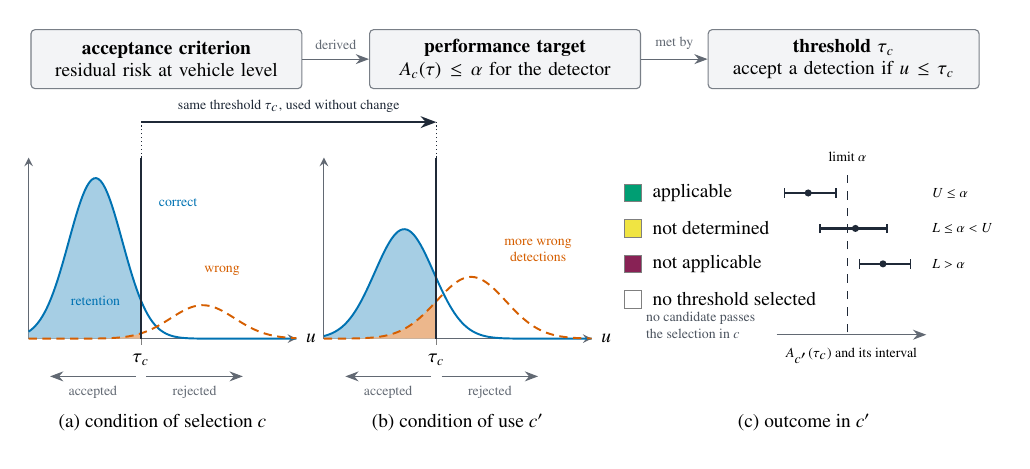
\begin{tikzpicture}[font=\scriptsize, >=Stealth,
  hbox/.style={draw=ink!60, fill=boxfill, rounded corners=1.5pt, align=center, inner sep=2pt, minimum height=7.5mm},
  lab/.style={font=\scriptsize, text=ink},
  sq/.style={draw=edge, line width=0.3pt, minimum size=2.2mm, inner sep=0pt}]
% ---------------- header chain
\node[hbox, text width=33mm] (ac) at (1.75,0) {\textbf{acceptance criterion}\\ residual risk at vehicle level};
\node[hbox, text width=33mm] (pt) at (6.05,0) {\textbf{performance target}\\ $A_c(\tau)\le\alpha$ for the detector};
\node[hbox, text width=33mm] (th) at (10.35,0) {\textbf{threshold $\tc$}\\ accept a detection if $u\le\tc$};
\draw[->, ink!70] (ac) -- node[above, font=\tiny]{derived} (pt);
\draw[->, ink!70] (pt) -- node[above, font=\tiny]{met by} (th);
% ---------------- panel (a): condition c
\def\gc#1#2#3{#1*exp(-((x-#2)^2)/(2*#3^2))/(#3*2.5066)}
\begin{axis}[at={(0cm,-3.55cm)}, anchor=south west, width=3.4cm, height=2.3cm, scale only axis,
  xmin=0, xmax=1, ymin=0, ymax=3.6, axis lines=left, ytick=\empty, xtick={0.42}, xticklabels={$\tc$},
  tick label style={font=\scriptsize}, axis line style={ink!70}, clip=false, samples=120, domain=0:1]
  \addplot[name path=ca, draw=corr, line width=0.7pt] {\gc{0.8}{0.25}{0.10}};
  \addplot[name path=wa, draw=wrng, line width=0.7pt, densely dashed] {\gc{0.2}{0.65}{0.12}};
  \path[name path=xa] (axis cs:0,0) -- (axis cs:1,0);
  \addplot[corr!35] fill between[of=ca and xa, soft clip={domain=0:0.42}];
  \addplot[wrng!45] fill between[of=wa and xa, soft clip={domain=0:0.42}];
  \draw[ink, line width=0.8pt] (axis cs:0.42,0) -- (axis cs:0.42,3.6);
  \node[font=\scriptsize, anchor=west] at (axis cs:1.0,0) {$u$};
  \node[font=\tiny, text=corr, anchor=west] at (axis cs:0.45,2.7) {correct};
  \node[font=\tiny, text=wrng, anchor=west] at (axis cs:0.62,1.35) {wrong};
  \node[font=\tiny, text=corr, align=center] at (axis cs:0.25,0.75) {retention};
  \draw[->, ink!70] (axis cs:0.40,-0.75) -- node[below, font=\tiny]{accepted} (axis cs:0.08,-0.75);
  \draw[->, ink!70] (axis cs:0.44,-0.75) -- node[below, font=\tiny]{rejected} (axis cs:0.80,-0.75);
\end{axis}
% ---------------- panel (b): condition c'
\begin{axis}[at={(3.75cm,-3.55cm)}, anchor=south west, width=3.4cm, height=2.3cm, scale only axis,
  xmin=0, xmax=1, ymin=0, ymax=3.6, axis lines=left, ytick=\empty, xtick={0.42}, xticklabels={$\tc$},
  tick label style={font=\scriptsize}, axis line style={ink!70}, clip=false, samples=120, domain=0:1]
  \addplot[name path=cb, draw=corr, line width=0.7pt] {\gc{0.6}{0.30}{0.11}};
  \addplot[name path=wb, draw=wrng, line width=0.7pt, densely dashed] {\gc{0.4}{0.55}{0.13}};
  \path[name path=xb] (axis cs:0,0) -- (axis cs:1,0);
  \addplot[corr!35] fill between[of=cb and xb, soft clip={domain=0:0.42}];
  \addplot[wrng!45] fill between[of=wb and xb, soft clip={domain=0:0.42}];
  \draw[ink, line width=0.8pt] (axis cs:0.42,0) -- (axis cs:0.42,3.6);
  \node[font=\scriptsize, anchor=west] at (axis cs:1.0,0) {$u$};
  
  \node[font=\tiny, text=wrng, align=center] at (axis cs:0.80,1.75) {more wrong\\ detections};
  \draw[->, ink!70] (axis cs:0.40,-0.75) -- node[below, font=\tiny]{accepted} (axis cs:0.08,-0.75);
  \draw[->, ink!70] (axis cs:0.44,-0.75) -- node[below, font=\tiny]{rejected} (axis cs:0.80,-0.75);
\end{axis}
\draw[ink, densely dotted] (1.428,-1.25) -- (1.428,-0.80);
\draw[ink, densely dotted] (5.178,-1.25) -- (5.178,-0.80);
\draw[->, ink, line width=0.6pt] (1.428,-0.80) -- node[above, font=\tiny]{same threshold $\tc$, used without change} (5.178,-0.80);
\node[font=\scriptsize] at (1.70,-4.62) {(a) condition of selection $c$};
\node[font=\scriptsize] at (5.45,-4.62) {(b) condition of use $c'$};
% ---------------- panel (c): outcome in c'
\begin{scope}[shift={(7.55,-3.55)}]
  \node[font=\scriptsize] at (2.30,-1.07) {(c) outcome in $c'$};
  % number line
  \def\xa{1.95} \def\xb{3.75} \def\al{2.85}
  \draw[->, ink!70] (\xa,0.05) -- (\xb+0.1,0.05);
  \node[font=\tiny, anchor=north] at (\xa+0.95,0.0) {$A_{c'}(\tc)$ and its interval};
  \draw[ink, dashed] (\al,0.08) -- (\al,2.15);
  \node[font=\tiny, anchor=south] at (\al,2.12) {limit $\alpha$};
  \foreach \y/\col/\name/\lo/\pt/\hi/\rule in {
     1.85/appc/applicable/2.05/2.35/2.70/{$U\le\alpha$},
     1.40/ndc/not determined/2.50/2.95/3.35/{$L\le\alpha<U$},
     0.95/nac/not applicable/3.00/3.30/3.65/{$L>\alpha$}}{
    \node[sq, fill=\col] at (0.12,\y) {};
    \node[anchor=west, font=\scriptsize] at (0.25,\y) {\name};
    \draw[ink, line width=0.9pt] (\lo,\y) -- (\hi,\y);
    \draw[ink, line width=0.6pt] (\lo,\y-0.06) -- (\lo,\y+0.06) (\hi,\y-0.06) -- (\hi,\y+0.06);
    \fill[ink] (\pt,\y) circle (0.045);
    \node[anchor=west, font=\tiny] at (3.80,\y) {\rule};
  }
  \node[sq, fill=ntc] at (0.12,0.50) {};
  \node[anchor=west, font=\scriptsize] at (0.25,0.50) {no threshold selected};
  \node[anchor=north west, font=\tiny, text=ink!80, align=left, inner sep=1pt] at (0.25,0.38) {no candidate passes\\ the selection in $c$};
\end{scope}
\end{tikzpicture}
\end{document}
